\documentclass[12pt]{article}
\usepackage[english]{babel}
\usepackage[utf8x]{inputenc}
\usepackage{amsmath}
\usepackage{graphicx}
\usepackage[colorinlistoftodos]{todonotes}
\usepackage{fancyhdr}
\usepackage[letterpaper, margin=.8in]{geometry}
\usepackage{sidecap}

\begin{document}

\begin{titlepage}

\newcommand{\HRule}{\rule{\linewidth}{0.5mm}} % Defines a new command for the horizontal lines

\center 
\textsc{\LARGE Marist College}\\[1.5cm]
\textsc{\Large ST: Deep Learning with TensorFlow}\\[0.5cm] 
\textsc{\large CMPT 469 Final Project}\\[0.5cm] 

\HRule \\[0.4cm]
{ \huge \bfseries Fast Artistic Style Transfer with TensorFlow}\\[0.4cm]
\HRule \\[1.5cm]
 
\begin{minipage}{0.4\textwidth}
\begin{flushleft} \large
\emph{Authors:}\\
Brian \textsc{Henderson} % Your name
\\
Sami \textsc{Ellougani} % Your name
\end{flushleft}
\end{minipage}
~
\begin{minipage}{0.4\textwidth}
\begin{flushright} \large
\emph{Professor:} \\
Dr. Pablo \textsc{Rivas} % Supervisor's Name
\end{flushright}
\end{minipage}\\[2cm]

{\large December 11, 2017}\\[2cm]

\begin{center}
  
\includegraphics[height=60mm]{visuals/tf.png}
\end{center}


\end{titlepage}

\begin{abstract}
 Artistic style transfer is a very interesting topic among the deep learning community. Training a neural network to be able to take such inspiring pieces of art and transfer that inspiration to any image, is truly a piece of art in itself. We take a look at some of the prominent research behind artistic style transfer, and go deep into their architecture to see how researchers from some of the finest institutions approach artistic style transfer. We took a liking towards \textit{Fast Style Transfer}, which allows for images to be styled in real time by pre-training a neural network for a specific style. Experimenting with different combinations of weights, we were able to produce quality images of the Marist College Hancock Center, using the artistic style of Francis Picabia's Udnie painting. Special thanks to Logan Engstrom, for developing the code architecture used during these experiments. \cite{Engstrom}
\end{abstract}

\section{Introduction}
This semester, we took on the challenge of learning how Deep Neural Networks work by delving deep into the implementation of an Artistic Style Transfer. An Artistic Style Transfer takes the style of one photo,
and puts it over another photo with the same artistic style. 

\begin{center}
  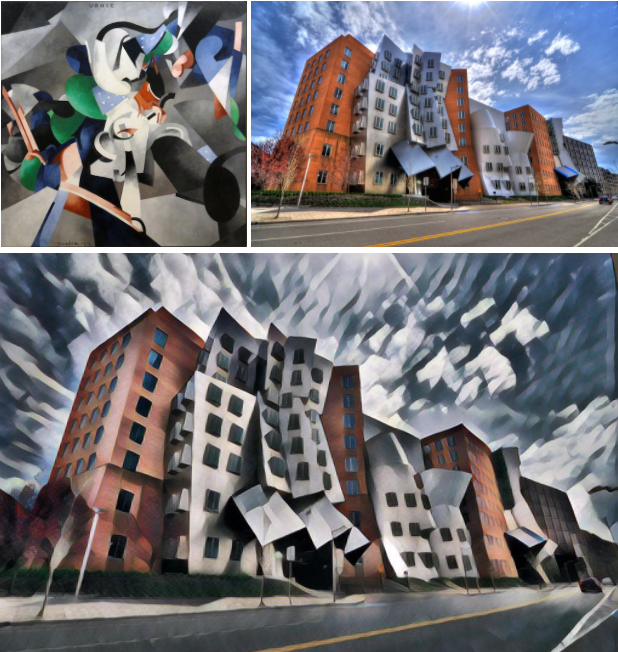
\includegraphics[height=75mm]{visuals/milestone_example.png}
\end{center}

Humans have mastered the skill to create unique visual experiences through composing a complex interplay between the content and style of an image.[2]
This seems like an almost impossible task to take a style from one photo to another, but to achieve this we will be using convolution neural networks to train styles. 
We've decided to apply the style transfer in real time, which will involve training networks with a designated style. We will use several resources as guides on how to begin TensorFlow implementation. Our objective is letting a user have the ability to upload upload various influential, abstract, and unique styles from different historical and modern time periods, select a pre-loaded style, and produce the output.


\section{Leon A. Gatys  A Neural Algorithm of Artistic Style}
\subsection{Interpretation of Convolutional Neural Networks}
Convolutional Neural Networks provide the best solution to handle image processing problems. Convolutional Neural Networks have several layers that process visual data in a hierarchical format.
This can then be helpful in retrieving data regarding what type of Artistic Style an image contains. Gatys goes into more depth about what a Convolution Neural Network consists of.
"Convolutional Neural Networks consist of layers of
small computational units that process visual information hierarchically in a feed-forward manner.
 Each layer of units can be understood as a collection of image filters, each of which
extracts a certain feature from the input image. Thus, the output of a given layer consists of
so-called feature maps: differently filtered versions of the input image" \cite{Gatys}

\subsection{Use of Convolution Neural Networks}
Very simply put, Convolution Neural Networks are useful for processing image data, which then helps us in the challenge of object recognition. 
Gatys states his reasoning for choosing a Convolution Neural Network for solving the issue of retrieving Artistic Style from a photograph. 
"When Convolutional Neural Networks are trained on object recognition, they develop a
representation of the image that makes object information increasingly explicit along the processing
hierarchy. Therefore, along the processing hierarchy of the network, the input image
is transformed into representations that increasingly care about the actual content of the image
compared to its detailed pixel values. We can directly visualize the information each layer
contains about the input image by reconstructing the image only from the feature maps in that
layer" \cite{Gatys} \\ \\
As we process the input image, we are able to get pixel values which we can then use to have a data representation of the Artistic Style the photograph has.
This then helps us towards our end goal of masking a secondary photo with the initial photo's Artistic Style. 

\subsection{Representation of Style}
Through this algorithm, we gain a representation of the style of an image
by including a feature that was originally used to capturing the texture of the photo. 
"By including the feature correlations of multiple layers, we obtain a stationary, multi-scale representation of the input
image, which captures its texture information but not the global arrangement." \cite{Gatys}

\begin{center}
    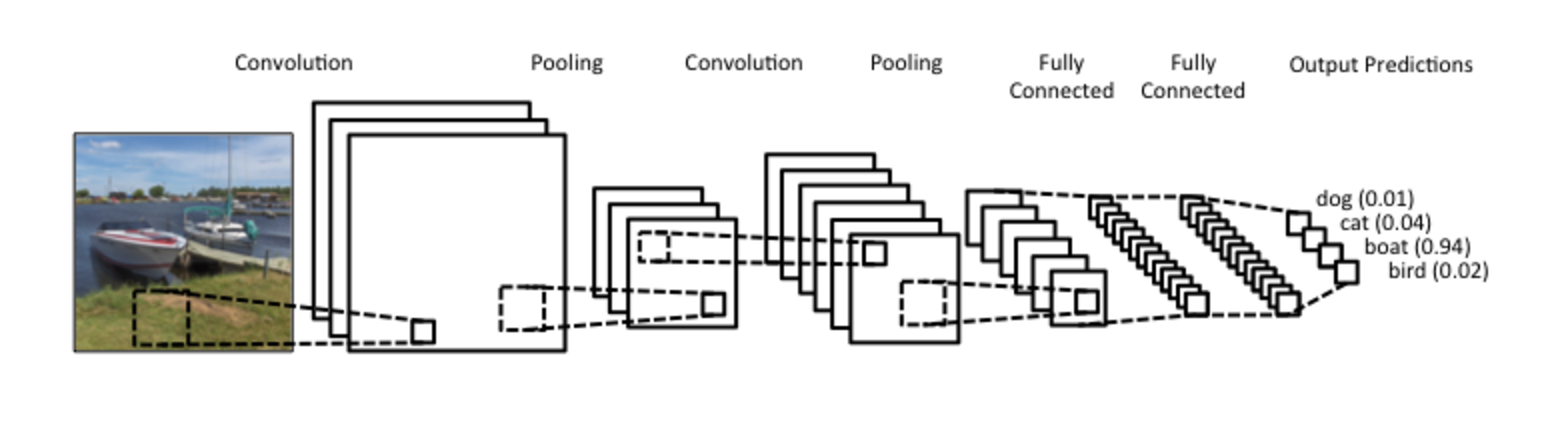
\includegraphics[height=60mm, width=160mm]{visuals/cnn.png}
\end{center}

%%%%%%%%%%%%

\section{Justin Johnson's Perceptual Losses for Real-Time Style Transfer and Super-Resolution}
Justin Johnson, \textit{Department of CS, Stanford University}, describes image transformation as a problem, "Where input image is transformed into an output image." \cite{Johnson} Recent and common solutions for this problem involve training feed-forward convoloutional neural networks, that produces the image by using a per-pixel loss from the output and original image. Successful images have also been generated by optimizing and defining perceptual loss functions that extract high-level functions from the pre-trained networks. Johnson introduces a hybrid concept of both approaches, suggesting the use of perceptual loss functions for training feed-forward networks as a solution for the image transformation problem. 

\subsection{Per-Pixel Feed-Forward and Perceptual Loss Functions}
Per-pixel feed forward functions are very effective and efficient, they produce the output image by differentiating the pixels between the ground truth image and the output image. However it does not fully capture perceptual differences. When comparing two identical images, one image offset by one pixel, although being perceptually analogous, they would be perceived very differently from a per-pixel function. Perceptual loss functions are very effective at producing high quality images, however they are also very time and resource consuming. Perceptual loss functions extract the high level features from pre-trained convolutional neural networks. The output image is produced from optimizing a loss function, which produces high quality images, however it takes much longer since it must also solve the optimization problem.

\subsection{Johnson's Hybrid Approach}
Both of the explained approaches to solving the image transformation problem have their strengths and weakness's, so Johnson proposes taking the strengths from both and combine them together. The networks are trained using perceptual loss functions that are dependant on the high-level features that have been trained in a loss network. The training is done in a feed-forward transformation network. This hybrid allows for network to be executed in real time, and distinguishes image similarities on a broader spectrum.

\subsection{Methodology Architecture}
Johnson's architecture is comprised of two fundamentals, the image transformation network and the loss function. The Image transformation network is a deep residual convoloutional neural network that is characterized by weights, and is trained using stochastic gradient decent that minimizes the weighted combination of loss functions. The loss network defines the feature reconstruction loss and style reconstruction loss, which measures the differences in the content and style between the images. The benefits of this methodology is that the convoloutional neural networks trained have already learned to encode the perceptual and semantic information that are measured in the loss functions. Johnson makes use of the pre-trained network as a fixed loss network to define the loss functions. The deep convoloutional transformation network is trained by the loss functions, which are also deep convoloutional networks. \cite{Johnson}


%%%%%%%%%%%%

\section{Dmitry Ulyanov’s Instance Normalization: The Missing Ingredient for Fast Stylization}

\subsection{One Small Change, Significant Improvement}
Dmitry Ulyanov and his team recognizes how a minor change in the stylization architecture in image transformation can result in significant qualitative improvements in the output image. They build upon the feed-forward stylization architecture by replacing the batch normalization  layers with instance normalization layers in the generator architecture. It is also kept at test time instead of freezing and simplifying them out as done in batch normalization. This process allows the normalization any instance specific contrast information, overall simplifying the generation of the output image and producing higher quality results.

\subsection{Trends and Observations}
Some trends and inferences that were observed in the experiments were that the network that was trained with only $16$ images produced higher quality results than the network trained with thousands of images. They ultimately found that the networks that were trained with smaller batches of images and stopped early in the training process produced better results. It was also observed and mentioned how the stylization should not be dependent on the contrast of the content image, since the output image's contrast should be similar to the content image.\cite{Ulyanov}
\\\\
By replacing the batch normalization with the instance normalization and applying at test time, the results are significantly more impressive. What this does is it prevents the instance specific mean and co-variance shift, resulting in a simpler learning process. \cite{Ulyanov}


%%%%%%%%%%%%


\section{Pre-trained VGG-19 Model}
\subsection{Visual Geometry Group}
The Visual Geometry Group is an academic group that focuses on computer vision at Oxford University. The Visual Geometry Group has several publications and set the bar high in the field
of visual recognition. They contribute in several areas of evaluation of Convolutional Neural Networks to increase improvement of image recognition.

\subsection{VGG-16/19 Model}
VGG-16/19 is a pre-trained model that has a rich feature representation for a wide variety of images. VGG-16/19 is pre-trained using the ImageNet database, which means that the model is trained on more than a million images. As a result, the model excels in object recognition for a wide variety of images. The difference between VGG-16/19 is the amount of layers that both models use. VGG-16 uses 16 layers, while VGG-19 uses 19 layers.

\subsection{ImageNet Database}
ImageNet is a current research effort to provide researchers and engineers the capability to access an image database. This image database is vast as it contains more than a million images.
ImageNet is organized according to the WordNet hierarchy. The images in ImageNet are categorized by a couple of words, called "synonym sets." There are more than 100,000 synonym sets in 
the WordNet database, and the majority of them are nouns. ImageNet provides on average 1000 images to illustrate each synonym set.


\subsection{Figure of VGG-19 Model}
\begin{center}
  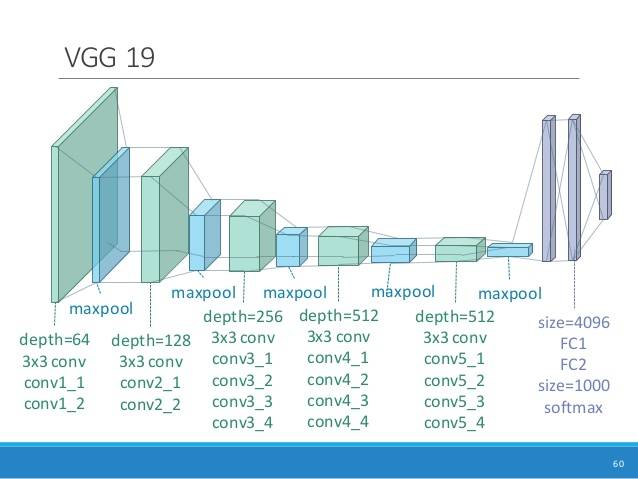
\includegraphics[height=75mm]{visuals/vgg-19.jpg}
\end{center}

\section{Microsoft Coco Data Set}

\subsection{About}
The Microsoft Coco data set contains over 330,000 images, and more than 200,000 of them being labeled. Item labeling is used for instance segmentation to aid object recognition. 

\subsection{Purpose of Coco Data Set}
This data set is used as well as the ImageNet database in our VGG-19 model for statistical analysis. "We present a detailed statistical analysis of the data set in comparison to PASCAL, ImageNet, and SUN. Finally, we provide baseline performance analysis for bounding box and segmentation detection results using a Deformable Parts Model."\cite{Coco}

\subsection{Figure of Annotation Pipeline}
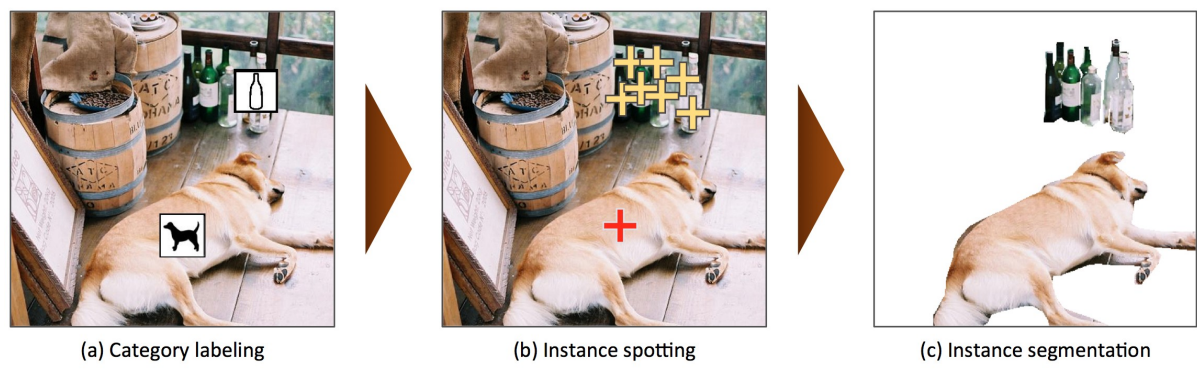
\includegraphics[height=75mm, width=160mm]{visuals/pipeline.png}

\section{Experiments}
Using Francis Picabia's 1913 painting, \textit{Udnie}, we ran several experiments transferring the style onto a picture of Marist College's Hancock Center. The purpose of the individualized experiments were diverse, however the general goal we were looking to accomplish was to modify the weights and see the affect on the output image. The code used for these experiments was developed by Logan Engstrom, \textit{Massachusetts Institute of Technology}, using technologies and concepts mentioned in this paper. \cite{Lengstrom} We installed TensorFlow from sources on a gCloud GPU instance, modified the weights, and analyzed the results.
\\
\\
*Experiments were run on Google’s gCloud Service using a NVIDIA Tesla K80 GPU
\\

\begin{minipage}[c]{0.3\textwidth}
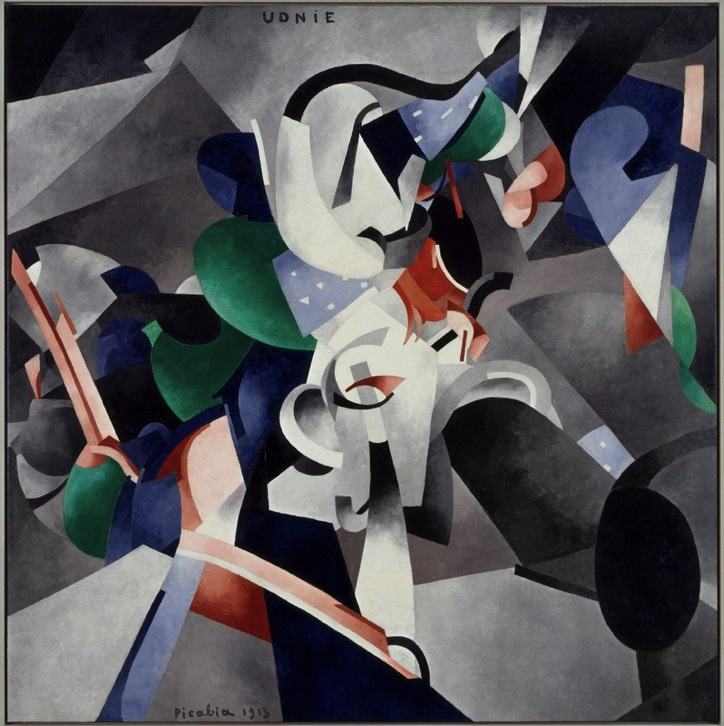
\includegraphics[height=50mm]{visuals/styles/udnie.jpg}
\end{minipage}
\begin{minipage}[c]{0.6\textwidth}
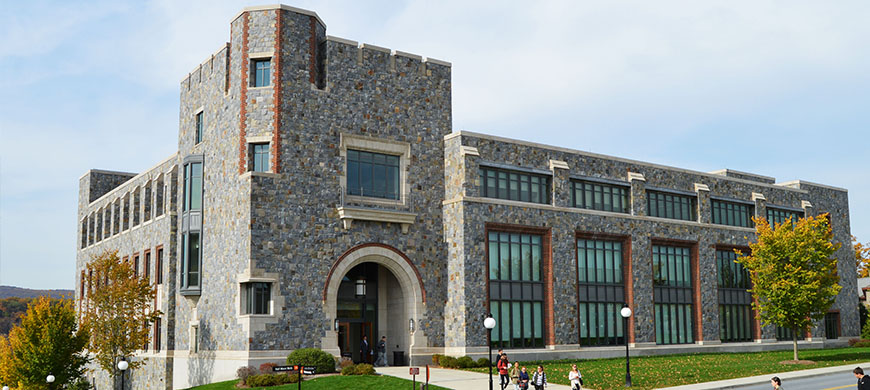
\includegraphics[height=50mm]{visuals/hancock.jpg}
\end{minipage}

\subsection{Experiment 00}
\subsubsection{Hypothesis} Get a base understanding of the weights and modify appropriately using the results of this experiment.
\subsubsection{Weights and Result}
\begin{minipage}[t]{0.4\textwidth}
\begin{tabular}{l l}
    \textbf{Epochs} &$3$     \\
    \textbf{Batch Size}     & $4$     \\
    \textbf{Content Weight} & $7.5e0$ \\
    \textbf{Learning Rate}  & $1e-3$  \\
    \textbf{Style Weight}   & $1e2$ \\
    \textbf{Completion Time}  & 24hrs  \
\vspace{3.5cm}\\
\end{tabular}
\end{minipage}
\begin{minipage}{0.1\textwidth}
\end{minipage}
\begin{minipage}[t]{0.6\textwidth}
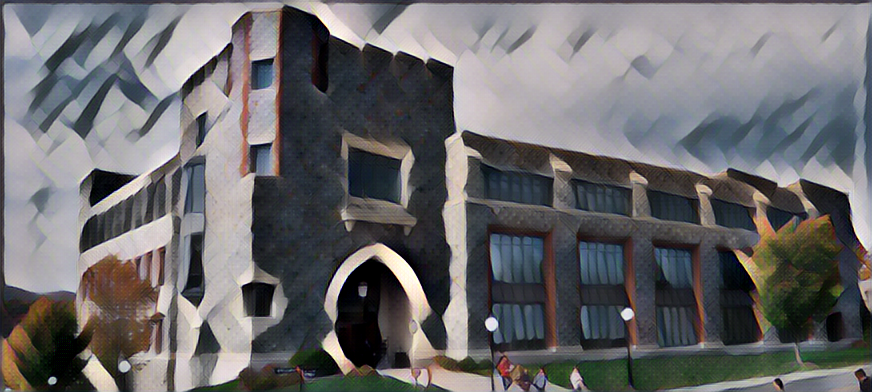
\includegraphics[height=50mm]{visuals/results/00.png}
\end{minipage} \vspace{-3cm}
\subsubsection{Analysis}
Overall, the first experiment was successful with the production of a quality image. The sky's portion of the image has abstract "clouds," giving the image a sharp look. Downside to this architecture is training time took a full 24 hours to complete.


\subsection{Experiment 01}
\subsubsection{Hypothesis} Attempt to decrease training time with one less epoch, but increased batch size. Also increase the content weight and learning rate at an attempt to have the output image a little more smoother.
\subsubsection{Weights and Result}
\begin{minipage}[t]{0.4\textwidth}
\begin{tabular}{l l}
    \textbf{Epochs} & $2$     \\
    \textbf{Batch Size}     & $20$     \\
    \textbf{Content Weight} & $1.5e1$ \\
    \textbf{Learning Rate}  & $1e-2$  \\
    \textbf{Style Weight}   & $1e2$ \\
    \textbf{Completion Time}  & 12hrs  \
\vspace{3.5cm}\\
\end{tabular}
\end{minipage}
\begin{minipage}{0.1\textwidth}
\end{minipage}
\begin{minipage}[t]{0.6\textwidth}
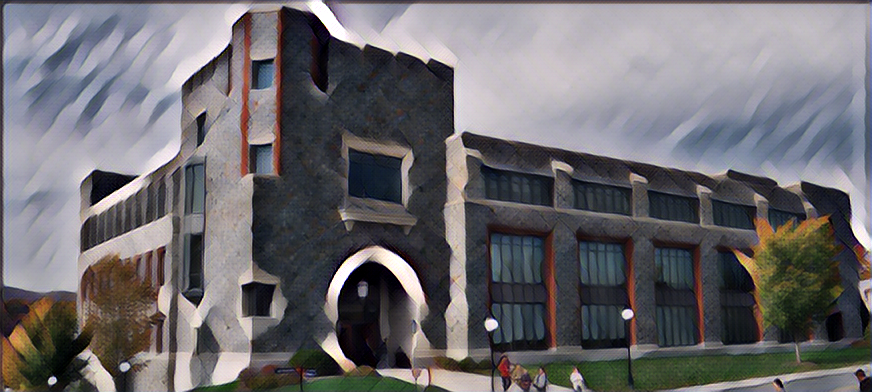
\includegraphics[height=50mm]{visuals/results/01.png}
\end{minipage} \vspace{-3cm}
\subsubsection{Analysis}
The training time for this network was 50\% less than the previous experiment and still produced a quality image. The style did smooth out as predicted, as seen in the sky.

\subsection{Experiment 02}
\subsubsection{Hypothesis} Try something different by increasing the style weight significantly and see what the result is.
\subsubsection{Weights and Result}
\begin{minipage}[t]{0.4\textwidth}
\begin{tabular}{l l}
    \textbf{Epochs}          & $2$     \\
    \textbf{Batch Size}      & $20$    \\
    \textbf{Content Weight}  & $1.5e1$ \\
    \textbf{Learning Rate}   & $1e-2$  \\
    \textbf{Style Weight}    & $1e4$   \\
    \textbf{Completion Time} & 12hrs \
\vspace{3.5cm}\\
\end{tabular}
\end{minipage}
\begin{minipage}{0.1\textwidth}
\end{minipage}
\begin{minipage}[t]{0.6\textwidth}
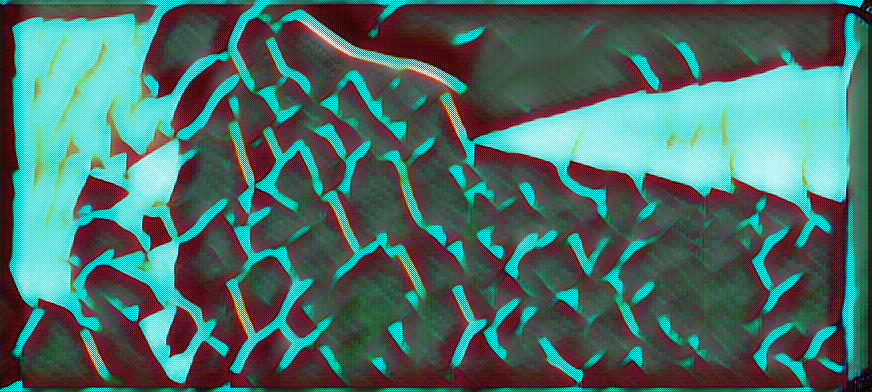
\includegraphics[height=50mm]{visuals/results/02.png}
\end{minipage} \vspace{-3cm}
\subsubsection{Analysis}
Not a successful experiment in respect to the quality of the output image, but definitely an interesting result.


\subsection{Experiment 03}
\subsubsection{Hypothesis} Revert the style weight back, and lower the content weight from experiment 01.
\subsubsection{Weights and Result}
\begin{minipage}[t]{0.4\textwidth}
\begin{tabular}{l l}
    \textbf{Epochs}          & $2$     \\
    \textbf{Batch Size}      & $20$    \\
    \textbf{Content Weight}  & $6e0$ \\
    \textbf{Learning Rate}   & $1e-2$  \\
    \textbf{Style Weight}    & $1e2$   \\
    \textbf{Completion Time} & 11hrs \
\vspace{3.5cm}\\
\end{tabular}
\end{minipage}
\begin{minipage}{0.1\textwidth}
\end{minipage}
\begin{minipage}[t]{0.6\textwidth}
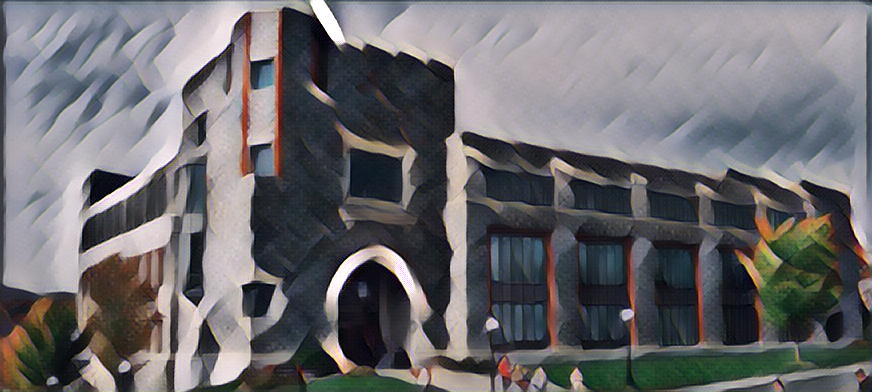
\includegraphics[height=50mm]{visuals/results/03.png}
\end{minipage} \vspace{-3cm}
\subsubsection{Analysis}
Successful experiment. Interesting in regards to the white glowing outline towards the top and left of the building.

\section{Different Styles}
After taking the poll during the class presentation, the majority of the class liked how Experiment 03's output image. We used the weights from this experiment, and decided to try it with different styles. Training each image takes around 11hrs, so we created a bash script, \texttt{runExpers.sh}, to execute the stylization four consecutive times. After two days, this is what we had for results!

\subsection{Dreaming In Gold}
\begin{minipage}[c]{0.3\textwidth}
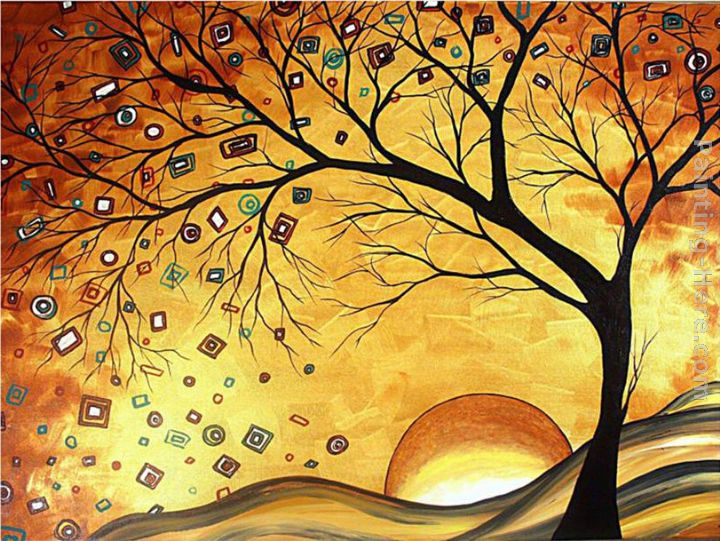
\includegraphics[height=50mm, width=50mm]{visuals/styles/dreaming-in-gold.jpg}
\end{minipage}
\begin{minipage}[c]{0.6\textwidth}
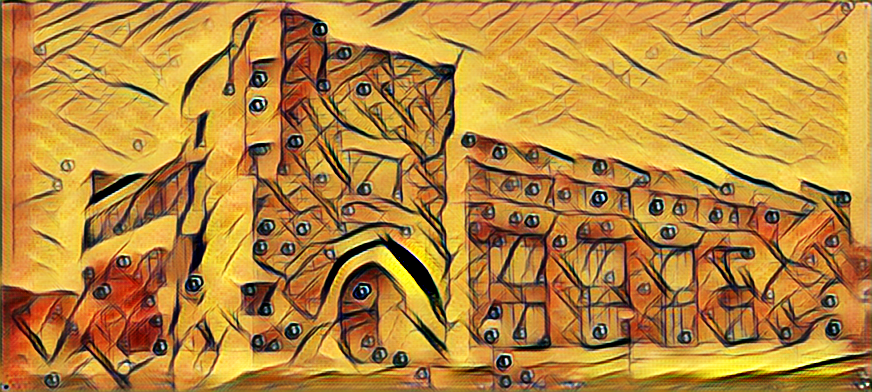
\includegraphics[height=50mm]{visuals/results/04.png}
\end{minipage}

\subsection{Once Only}
\begin{minipage}[c]{0.3\textwidth}
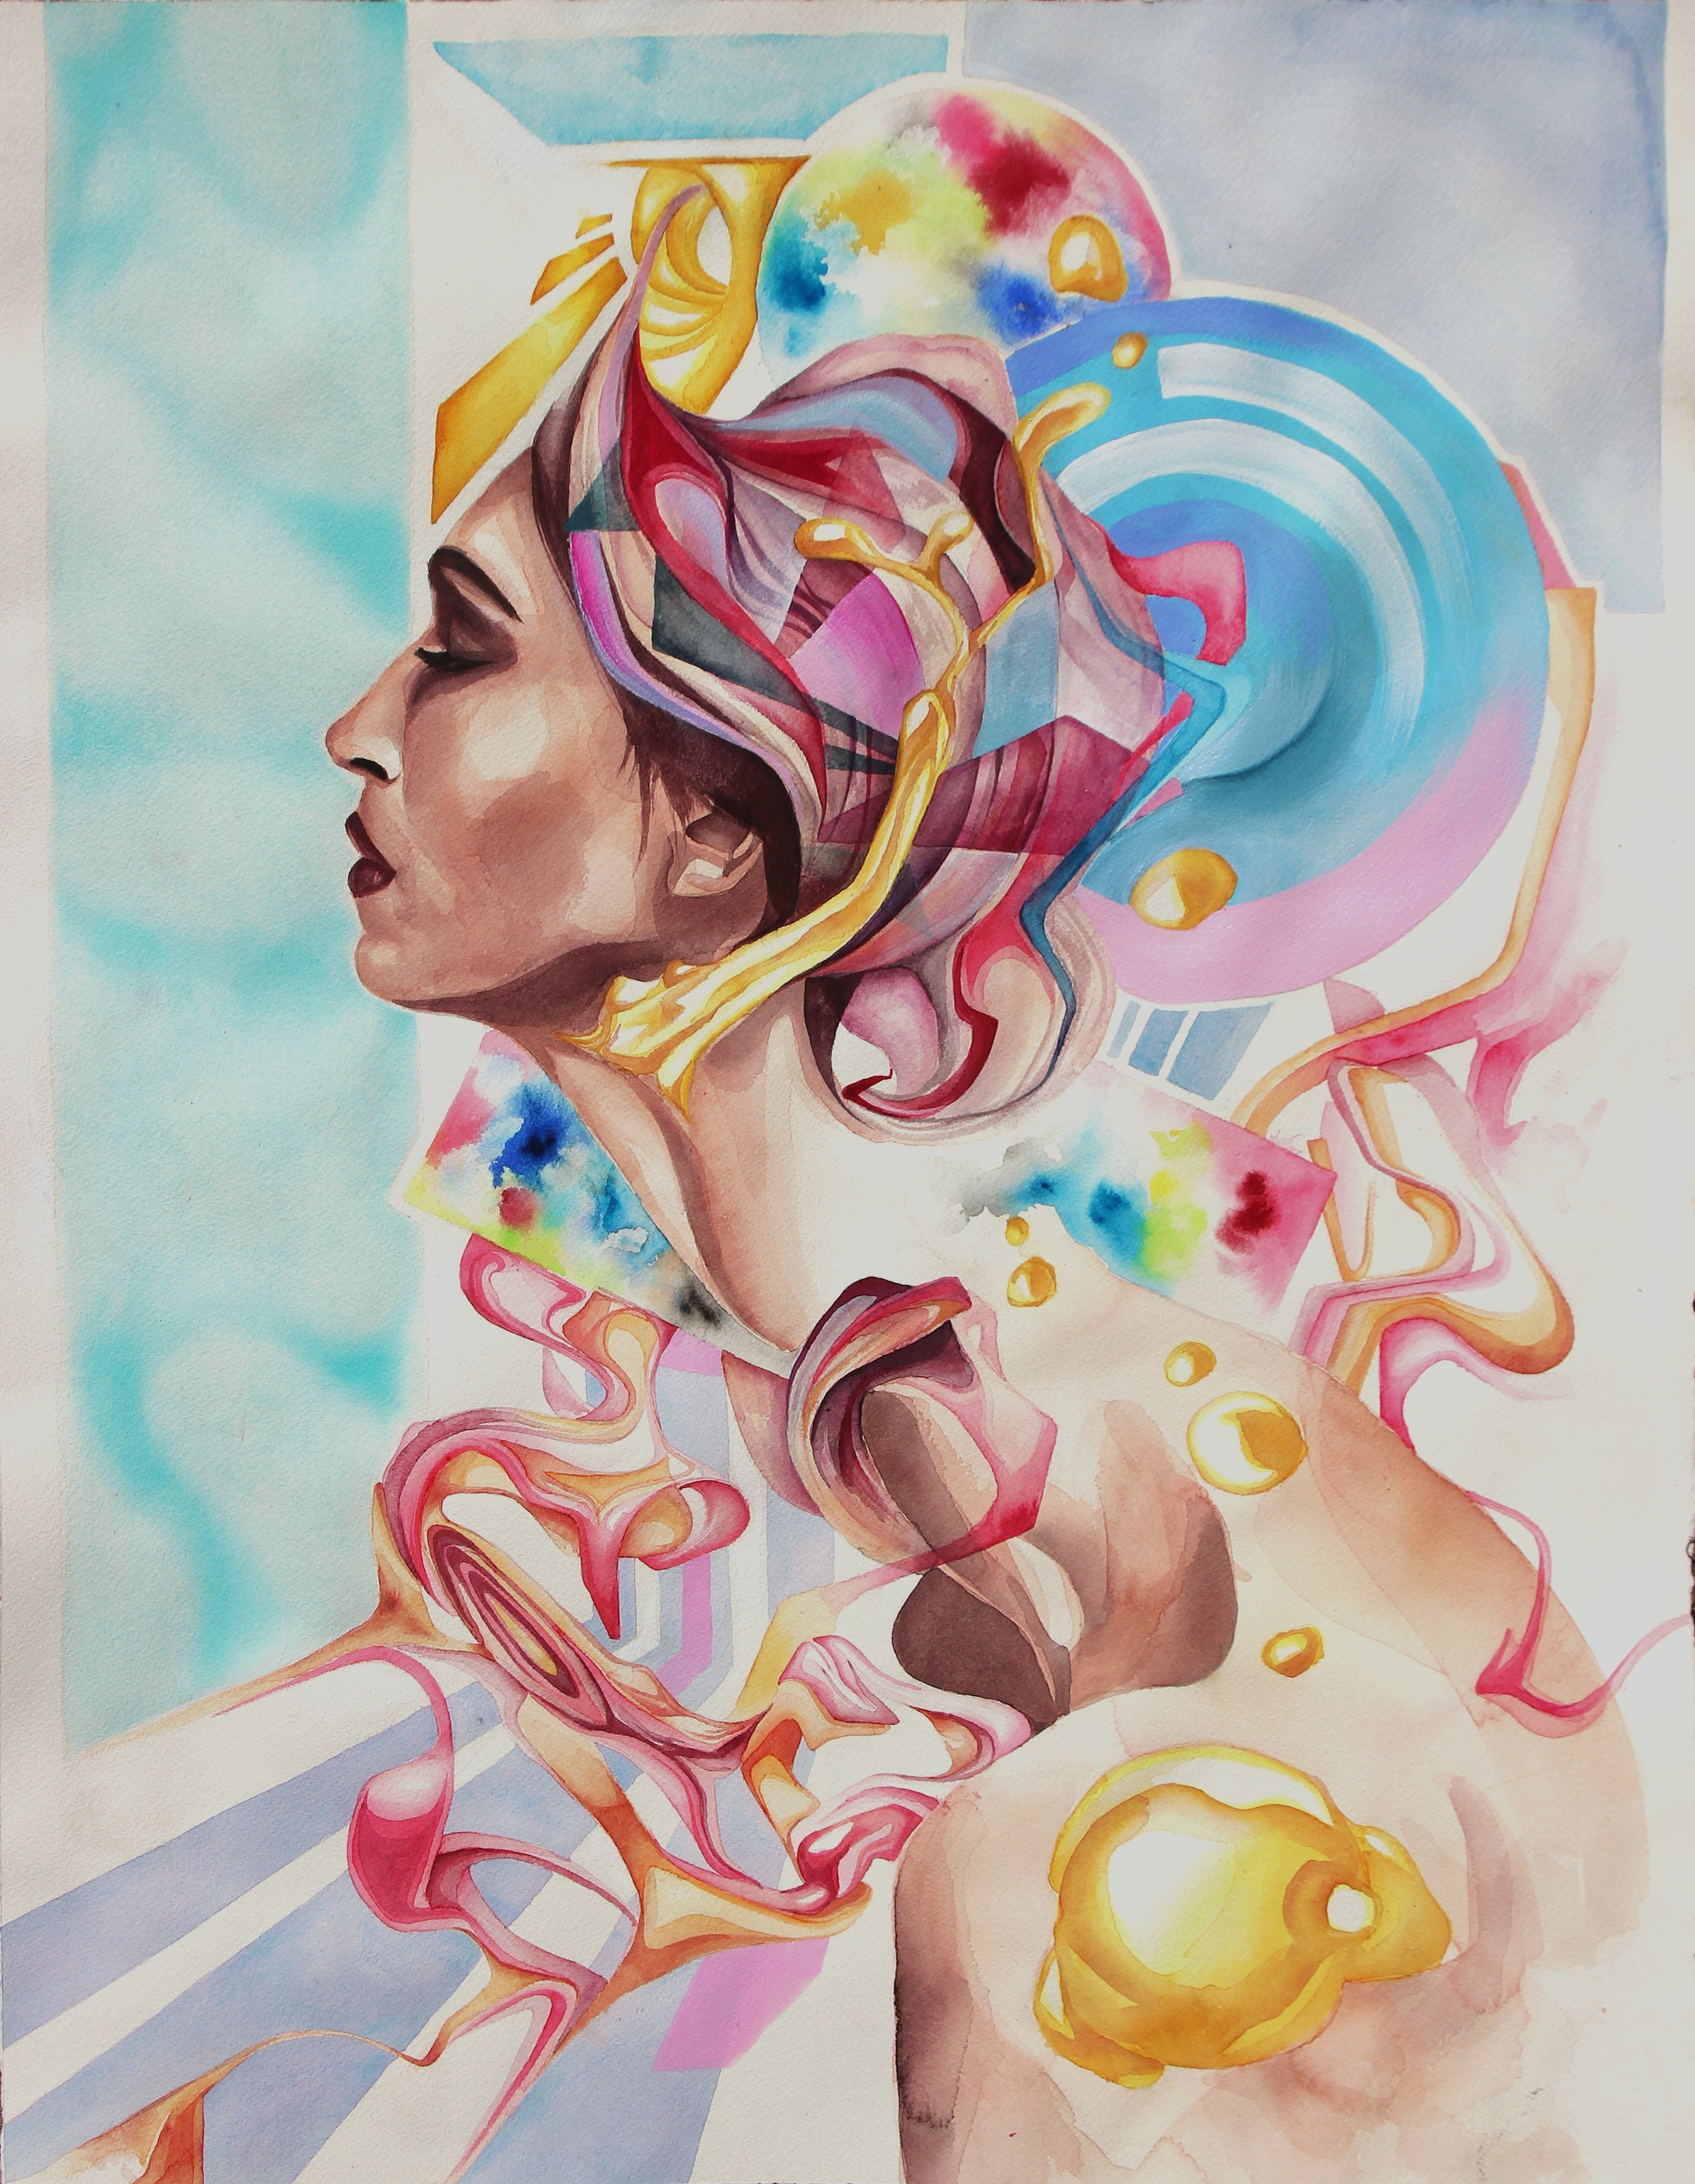
\includegraphics[height=50mm, width=50mm]{visuals/styles/once-only.jpg}
\end{minipage}
\begin{minipage}[c]{0.6\textwidth}
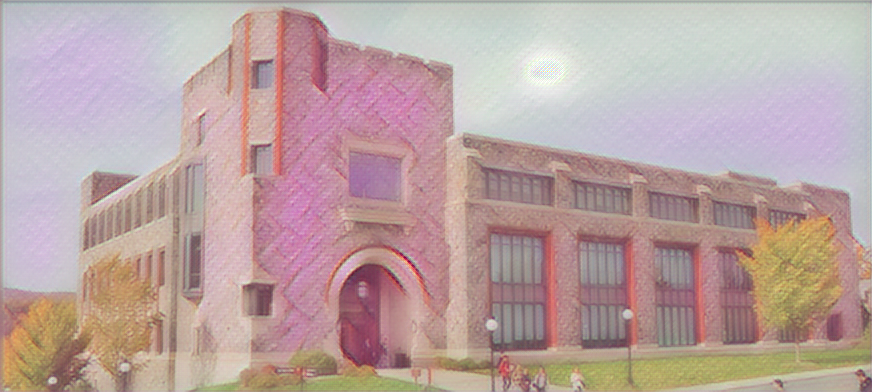
\includegraphics[height=50mm]{visuals/results/05.png}
\end{minipage}

\subsection{Starry Night}
\begin{minipage}[c]{0.3\textwidth}
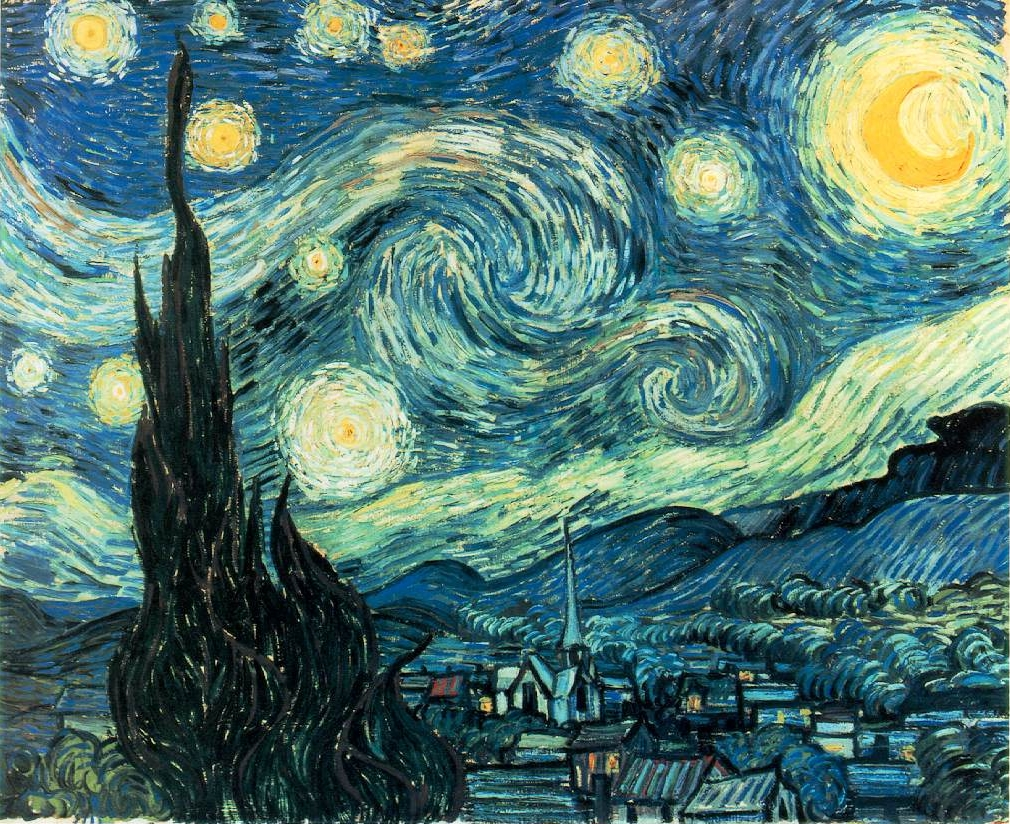
\includegraphics[height=50mm, width=50mm]{visuals/styles/starry-night.jpg}
\end{minipage}
\begin{minipage}[c]{0.6\textwidth}
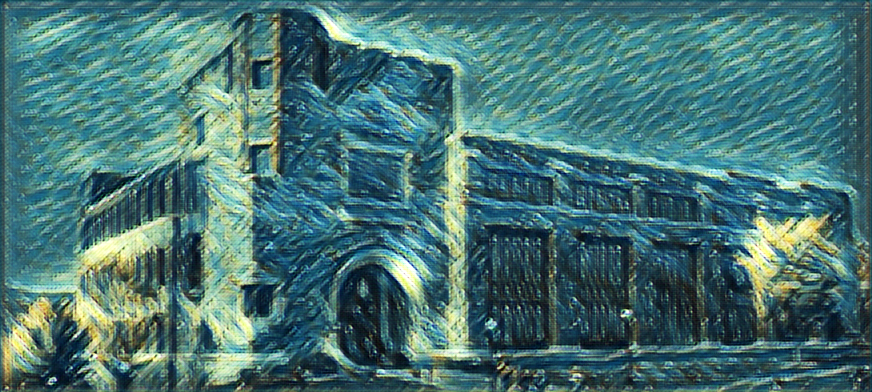
\includegraphics[height=50mm]{visuals/results/06.png}
\end{minipage}

\subsection{Cafe Terrace}
\begin{minipage}[c]{0.3\textwidth}
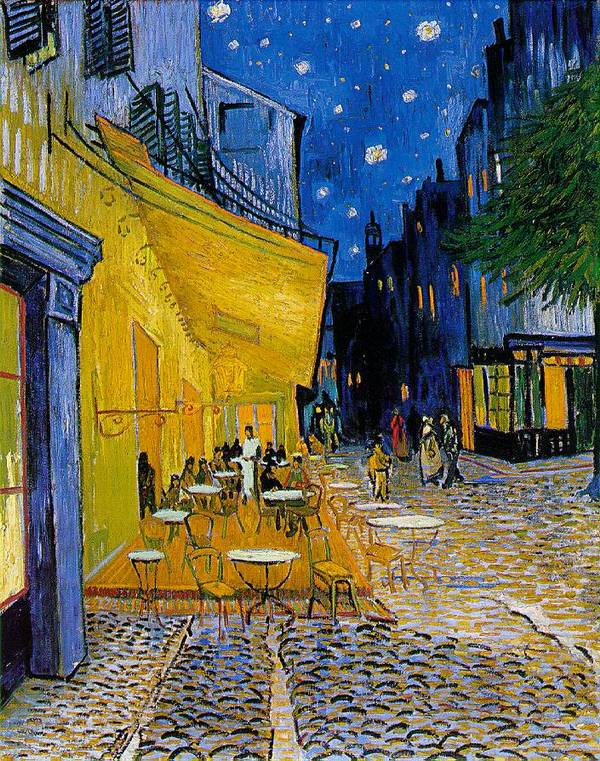
\includegraphics[height=50mm, width=50mm]{visuals/styles/cafe-terrace-at-night.jpg}
\end{minipage}
\begin{minipage}[c]{0.6\textwidth}
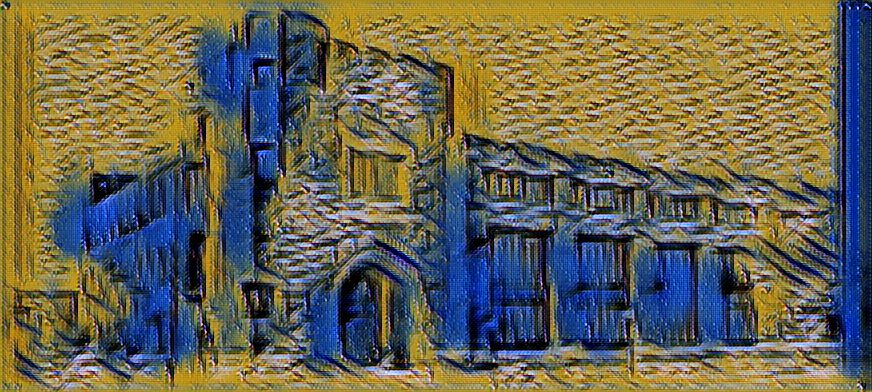
\includegraphics[height=50mm]{visuals/results/07.png}
\end{minipage}

\subsection{Analysis}
We were excited to see how this set of experiments were going to turn out. Although the output image is not as cleary defined as the Udnie version, the images were very interesting. We were hoping to have a little higher quality output image, however we realized something. Art is unique, and each piece requires the special attention to detail that was put into it by the artist. Overall, we were pleased with the results, (besides Cafe Terrace), the images were interesting to look at and has certainly sparked interest and curiosity in this area of deep learning.

\section{Conclusion}
Deep Neural Networks are very interesting, they can do amazing things, human like things. Training a computer to be able to take a piece of work that such a gifted human produced, and being able to recreate it and extend that persons legacy, is truly incredible. It has also shown to be very complex, every piece of art is unique in its own way and requires attention to even the smallest details. Gatys outlines the use of convoloutional neural networks very well, and gave other researchers clarity and the inspiration to look into this topic. Jutin Johnson and his team built upon Gatys work and were able to make a style network that ran in real time, using his hybrid approach. Ulyanov noticed how he could improve upon existing architectures by making one small modification. All these factors led the creation of the code that was used in the experiments we ran using the artistic style of the famed Udnie painting, and our very own Marist College Hancock Center, as well as the additional experiments we ran using various other works of art.

\newpage
\medskip
\begin{thebibliography}{9}
\bibitem{Gatys} 
Gatys, Leon A., et al.
\textit{ “A Neural Algorithm of Artistic Style.”}.  [1508.06576] A Neural Algorithm of Artistic Style, 2 Sept. 2015, arxiv.org/abs/1508.06576.\

\bibitem{Coco} 
Lin, Tsung-Yi, et al. 
\textit{ “Microsoft COCO: Common Objects in Context.” }.  [1405.0312] Microsoft COCO: Common Objects in Context, 21 Feb. 2015, arxiv.org/abs/1405.0312.

\bibitem{Johnson}
Johnson, Alahi, Fei-Fei, et al.
\textit{"Perceptual losses for real-time style transfer and super-resolution."}. Perceptual losses for real-time style transfer and super-resolution. , 2016, http://cs.stanford.edu/people/jcjohns/eccv16/

\bibitem{Ulyanov}
Ulyanov, Vedaldi, Lempitsky, et al.
\textit{"Instance Normalization: The Missing Ingredient for Fast Stylization"}. [1607.08022] Instance Normalization: The Missing Ingredient for Fast Stylization, 7 Jun. 2017, arxiv.org/abs/1607.08022

\bibitem{Lengstrom}
Engstrom, et al.
\textit{Fast Style Transfer in TensorFlow}. Fast Style Transfer in TensorFlow, 2016, github.com/lengstrom/fast-style-transfer/

\end{thebibliography}

\end{document}

\end{document}   